\documentclass[12pt]{extarticle}
%Some packages I commonly use.
\usepackage[english]{babel}
\usepackage{graphicx}
\usepackage{framed}
\usepackage[normalem]{ulem}
\usepackage{amsmath}
\usepackage{amsthm}
\usepackage{amssymb}
\usepackage{multirow}
\usepackage{multicol}
\usepackage{adjustbox}
\usepackage{amsfonts}
\usepackage{enumerate}
\usepackage[utf8]{inputenc}
\usepackage[top=1 in,bottom=1in, left=1 in, right=1 in]{geometry}
\usepackage{hyperref}
\usepackage{xcolor}
\usepackage{rotating} 
\usepackage{booktabs}
\usepackage{subfig}
\usepackage[strict]{chngpage}
\usepackage{textcomp}
%\usepackage{subcaption}
%\usepackage[sc]{caption}
\usepackage{float}
\usepackage{soul}   % testo barrato

%A bunch of definitions that make my life easier
\newcommand{\matlab}{{\sc Matlab} }
\newcommand{\cvec}[1]{{\mathbf #1}}
\newcommand{\rvec}[1]{\vec{\mathbf #1}}
\newcommand{\ihat}{\hat{\textbf{\i}}}
\newcommand{\jhat}{\hat{\textbf{\j}}}
\newcommand{\khat}{\hat{\textbf{k}}}
\newcommand{\minor}{{\rm minor}}
\newcommand{\trace}{{\rm trace}}
\newcommand{\spn}{{\rm Span}}
\newcommand{\rem}{{\rm rem}}
\newcommand{\ran}{{\rm range}}
\newcommand{\range}{{\rm range}}
\newcommand{\mdiv}{{\rm div}}
\newcommand{\proj}{{\rm proj}}
\newcommand{\R}{\mathbb{R}}
\newcommand{\N}{\mathbb{N}}
\newcommand{\Q}{\mathbb{Q}}
\newcommand{\Z}{\mathbb{Z}}
\newcommand{\<}{\langle}
\renewcommand{\>}{\rangle}
\renewcommand{\emptyset}{\varnothing}
\newcommand{\attn}[1]{\textbf{#1}}
\theoremstyle{definition}
\newtheorem{theorem}{Theorem}
\newtheorem{corollary}{Corollary}
\newtheorem*{definition}{Definition}
\newtheorem*{example}{Example}
\newtheorem*{note}{Note}
\newtheorem{exercise}{Exercise}
\newcommand{\bproof}{\bigskip {\bf Proof. }}
\newcommand{\eproof}{\hfill\qedsymbol}
\newcommand{\Disp}{\displaystyle}
\newcommand{\qe}{\hfill\(\bigtriangledown\)}
\setlength{\columnseprule}{1 pt}
\newcommand*\rfrac[2]{{}^{#1}\!/_{#2}}

\begin{document}

\begin{figure}[]
\centering
{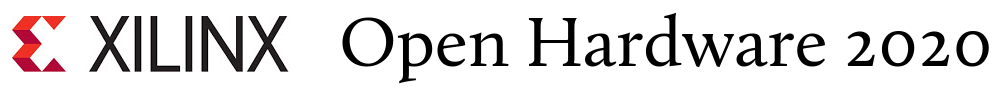
\includegraphics[width=1.0\textwidth]{images/xilinxoh.png}}
\end{figure}

\begin{figure}[]
\centering
{
\includegraphics[width=.15\textwidth]{images/Padova.png}}
\end{figure}

\begin{center}
{\large{U}\normalsize{NIVERSITÀ DEGLI}\large{ S}\normalsize{TUDI DI}\large{ P}\normalsize{ADOVA}}\\
% \textit{Corso di Dottorato in Physics}\\
% {\small{Anno accademico 2018-2019}}\\
\textit{ }\\
\textbf{\large{Documents Submission for Xilinx Open Hardware 2020}}\\
\textit{ }\\
\textit{ }\\
\textit{ }\\
\textit{ }\\
\textit{\Large{Report on the 'NCO based CDR implementation in FPGA'}} \\
\textit{ }\\
\textit{ }\\
\textit{ }\\
\textit{ }\\
\textbf{Team number: xohw20\_203}\\
\textit{ }\\
Team Partecipant: Filippo Marini$^1$\\
\textit{ }\\
Team Supervisor: Dr. Ing. Marco Bellato$^2$\\
\textit{ }\\
\end{center}

\textit{ }\\
$1$: Universita' degli Studi di Padova, INFN Padova. \textit{filippo.marini@pd.infn.it}\\
$2$: INFN Padova. \textit{marco.bellato@pd.infn.it}\\
\newpage

\section*{Abstract}
The capability to extract timing informations out of a serial data stream to
decode the incoming informations has become a very common requirement. To sample
the incoming data, the receiver usually relies on a Clock and Data Recovery
(CDR) chip, which generates a clock signal at the corresponding sampling
frequency, phase-aligned to the data. Modern physics experiment have often this
same requirement, where perhaps thousands of boards receive uncorrelated data
and it's up to them to decode the messages. For that reason, the presence of a
CDR on-board is usually mandatory. Present readout systems in physics
experiments usually rely on FPGAs to receive and transmit data at high rate to
high capaicity DAQ systems; exploting FPGAs to recover timing information from
streamed data is therefore beneficial for a number of reasons, including power
consumption and cost reduction. The design is based on two components: a
Numerically-Controlled Oscillator (NCO), in order to create a controlled
frequency clock signal, and a digital Phase Detector (PD) to match the clock
frequency with the data rate. NCOs are often coupled with a Digital to Analog
Converter (DAC) to create Direct Digital Synthesizers (DDS), which are able to
produce analog waveforms of any desired frequency. In the presented case, the
NCO generates a digital clock signal of an arbitrary frequence, while the PD
manages this frequency by intercepting any shifting on the relative phase
between the clock and the data. The report presents the implemented CDR design,
the limitations and the challenges involved, possible fields of application in
actual physics experiments and, finally, some results.
\end{document}